\chapter{Réseau de neurones \\(Thibault \& Quentin)}

L'élement central du logiciel d'OCR devait être en place dès la première
soutenance, et nécessitait une implémentation assez flexible pour passer d'un
apprentissage d'une simple fonction XOR à la reconnaissance de caractères. Le
réseau construit avait donc une architecture totalement modulaire, ce qui a par
la suite facilité les tests ainsi que le développement pour la dernière
soutenance.

L'aspect technique a été découpé en plusieurs parties :

\begin{itemize}
    \item Réflexion théorique de l'implémentation et des besoins.
    \item Implémentation des structures fondamentales : matrices, couches,
        réseau.
    \item Implémentation des fonctions principales du réseau : propagation,
        apprentissage.
    \item Améliorations diverses pour un apprentissage plus conséquent :
        mini-batch, entropie croisée, régularisation.
\end{itemize}

Chaque étape de développement a nécessité des tests avant de passer à l'étape
suivante, afin de s'assurer au maximum de la stabilité des fondements de notre
réseau. Nous avons ainsi mis en place un module de tests au sein du projet, que
l'on peut utiliser avec l'option \mintinline{text}{--test}.

\section{Architecture}

Notre réseau de neurones se compose des trois structures suivantes :

\begin{myminted}{neural\_network.h}
struct Layer
{
    size_t nb_neurons;
    struct Matrix *in;
    struct Matrix *out;
    struct Matrix *weight;
    struct Matrix *bias;
    struct Matrix *delta;
};

struct Network
{
    size_t nb_layers;
    struct Layer *layers;
};
\end{myminted}

\begin{myminted}{matrix.h}
struct Matrix
{
    size_t nb_rows;
    size_t nb_cols;
    float *mat;
};
\end{myminted}

\newpage

La création d'un réseau de neurones avec cette structure nécessite uniquement de
préciser le nombre de couches, ainsi que leurs tailles respectives. Par exemple
pour notre réseau apprenant la fonction XOR le code est :

\vspace{1em}

\begin{myminted}{xor\_network.c}
size_t layers_size[] = {2, 3, 2};
struct Network *network = network_alloc(3, layers_size);
...
network_free(network);
\end{myminted}

\vspace{2em}

Ceci nous crée le réseau de neurones suivant :

% http://www.texample.net/tikz/examples/neural-network/
\def\layersep{2.5cm}
\vspace{1cm}
\begin{center}
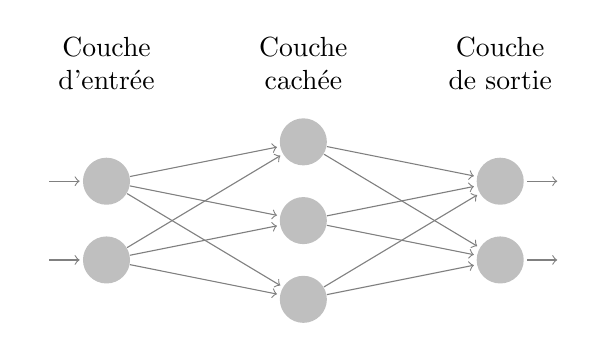
\begin{tikzpicture}[shorten >=1pt,->,draw=black!50, node distance=\layersep]
    \tikzstyle{every pin edge}=[<-,shorten <=1pt]
    \tikzstyle{neuron}=[circle,fill=black!25,minimum size=17pt,inner sep=0pt]
    \tikzstyle{annot}=[text width=4em, text centered]

    % Draw the input layer nodes
    \node[neuron, pin=left:] (I-1) at (0,-1.5) {};
    \node[neuron, pin=left:] (I-2) at (0,-2.5) {};

    % Draw the hidden layer nodes
    \node[neuron] (H-1) at (2.5, -1) {};
    \node[neuron] (H-2) at (2.5, -2) {};
    \node[neuron] (H-3) at (2.5, -3) {};

    % Draw the output layer node
    \node[neuron,pin={[pin edge={->}]right:}] (O-1) at (5, -1.5) {};
    \node[neuron,pin={[pin edge={->}]right:}] (O-2) at (5, -2.5) {};

    % Connect every node in the input layer with every node in the
    % hidden layer.
    \foreach \source in {1,...,2}
        \foreach \dest in {1,...,3}
            \path (I-\source) edge (H-\dest);

    % Connect every node in the hidden layer with the output layer
    \foreach \source in {1,...,3}
    {
        \path (H-\source) edge (O-1);
        \path (H-\source) edge (O-2);
    }

    % Annotate the layers
    \node[annot,above of=H-1, node distance=1cm] (hl) {Couche cachée};
    \node[annot,left of=hl] {Couche d'entrée};
    \node[annot,right of=hl] {Couche de sortie};
\end{tikzpicture}
\end{center}

\newpage

\section{Propagation}

L'abstraction de l'architecture du réseau à l'aide de matrice aide grandement
l'implémentation de la propagation, où chaque formule se résume simplement par
des opérations matricielles basiques.

Pour chaque formule, $l$ représente une couche quelconque du réseau et $L$ la
dernière couche.

\subsection{Propagation avant}

Lorsque l'entrée du réseau est initialisée, la propagation avant se charge de
calculer couche par couche la sortie du réseau :

$in^l = weight^l \cdot out^{l-1} + bias^l$

$out^l = \sigma (in^l)$

Afin de faire tendre le résultat vers 0 lorsqu'il est faible ou vers 1 lorsqu'il
est élevé, on applique la fonction sigmoid pour obtenir une sortie d'une couche
continue entre 0 et 1.

\begin{figure}[H]
    \centering
    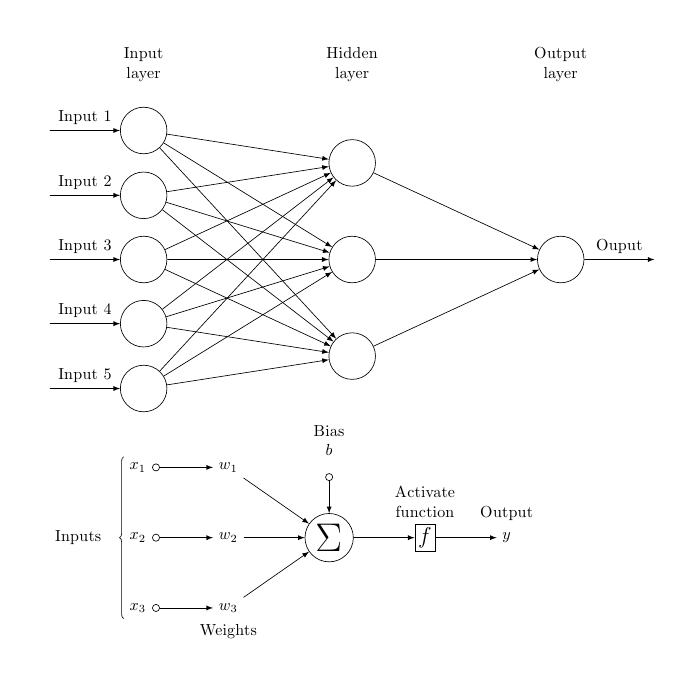
\includegraphics[width=0.6\textwidth]{network_forward}
\end{figure}

\subsection{Calcul d'erreur}

La seconde étape est de calculer l'erreur de sortie de notre réseau par rapport
à un résultat $y$ attendu. C'est ce calcul d'erreur qui va nous permettre par la
suite d'ajuster les poids et les biais du réseau lors de la rétropropagation.

$delta^L = out^L − y$

\subsection{Rétropropagation}

Enfin, il est nécessaire de propager en arrière le calcul d'erreur de la
dernière couche à la première :

$delta^l = ((weight^{l+1})^T \cdot delta^{l+1}) \odot \sigma '(in^l)$

\begin{figure}[H]
    \centering
    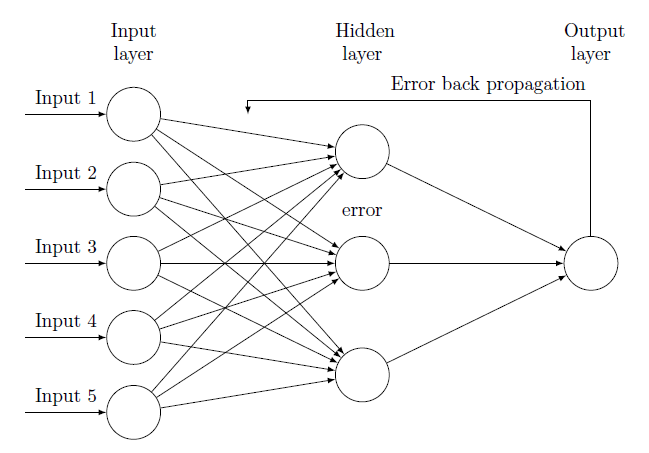
\includegraphics[width=0.7\textwidth]{network_backward}
\end{figure}

\newpage

\section{Apprentissage}

Pour l'apprentissage du réseau de neurones, l'\textbf{algorithme du gradient} a
été appliqué. Dans l'idée de rester sur une architecture modulaire, il fallait
généraliser le format des exemples donnés pour entraîner le réseau, afin que ce
dernier puisse aussi bien apprendre à partir de résultats d'un XOR que des
pixels d'une image. Pour cela, nous avons utilisé à nouveau notre abstraction de
matrice pour construire les deux structures suivantes :

\begin{myminted}{dataset.h}
struct ExampleData
{
    struct Matrix *in;
    struct Matrix *out;
};

struct Dataset
{
    size_t nb_examples;
    struct ExampleData *examples;
};
\end{myminted}

La structure \mintinline{c}{Dataset} permet ainsi de contenir n'importe quel
type de jeu de données. Pour l'apprentissage du réseau nous en aurons besoin de
trois types, tous gérés de la même façon à l'aide de la structure
\mintinline{c}{Dataset} :

\begin{itemize}
    \item \textbf{entraînement} : le jeu de données utilisé pour ajuster les
        poids et biais du réseau lors de l'apprentissage.
    \item \textbf{validation} : permet d'ajuster les paramètres internes du
        réseau (coefficient d'apprentissage, taux de régression, etc.) en
        utilisant une évaluation non biaisée du réseau.
    \item \textbf{test} : mesure finale non biaisée de l'efficacité du réseau de
        neurones sur un jeu de données.
\end{itemize}

Les formules de l'algorithme de gradient pour mettre à jour les poids et les
biais sont :

$weight^l = (1 - \frac{\eta\lambda}{n}) weight^l - \frac{\eta}{m} \displaystyle\sum^m{delta^l \cdot (out^{l-1})^T}$

$bias^l = bias^l - \frac{\eta}{m} \displaystyle\sum^m{delta^l}$

Où $\eta$ est le coefficient d'apprentissage, $\lambda$ le coefficient de
régression, $n$ la taille totale du jeu d'entraînement, et $m$ la taille du jeu
de données utilisé actuellement.

Pour la première soutenance, appliquer des sommations sur les $m$ exemples
n'était pas gênant puisque la fonction XOR est constituée uniquement de 4
exemples (correspondant à la table de vérité). En revanche, pour le jeu de
données comprenant plusieurs milliers d'images, il est nécessaire de découper
notre ensemble de données en plus petits sous-ensembles : c'est la méthode du
\textit{mini-batch gradient descent}.

À chaque étape de l'algorithme du gradient, notre jeu de données d'évaluation
est mélangé aléatoirement, et découpé en mini-batch de taille $m$.
L'entraînement et la modification des poids et des biais se fera donc sur ces
jeux de données plus petits, ce qui permet un apprentissage bien plus efficace.

La régularisation joue un rôle dans le calcul des modifications des poids, et
permet d'éviter à notre réseau de neurones l'effet de sur-apprentissage sur les
données d'entraînement. La méthode employée est celle de régularisation de
norme L2, où les paramètres extrêmes de notre modèle sont pénalisés afin
d'éviter une complexité qui tombe dans le sur-apprentissage.

\newpage

\section{Initialisation des valeurs du réseau}

L'initialisation des poids et des biais peut jouer un rôle assez important dans
l'apprentissage futur du réseau. Utiliser une loi normale de moyenne 0 et
d'écart-type 1 est une approche très efficace pour l'initialisation, d'autant
plus si l'on utilise la loi normale tronquée pour les poids (en fonction de
l'inverse de la racine carrée de la taille d'entrée de la couche).

La question se pose maintenant de comment obtenir une loi normale en C, car la
librairie standard ne fournit pas de tels outils. De nombreux algorithmes et
théorèmes mathématiques existent pour obtenir une loi normale. La méthode
retenue est celle de Marsaglia consistant à générer des paires de points
aléatoirement dans un carré jusqu'à ce qu'une condition sur les coordonnées soit
vérifiée. Cet algorithme est aussi celui implémenté dans la libstdc++ de GNU GCC
depuis le C++11.

\section{Jeu d'images}

Plusieurs jeux d'images sont déjà disponibles sur Internet, mais la plupart sont
utilisés pour des recherches avancées en traitement d'image et contiennent bien
plus d'informations que nécessaires pour notre utilisation. Nous avons décidé de
générer nos propres données ce qui nous donne un réel contrôle sur ces
dernières.

Dans un premier temps, nous étions partis sur un script Bash générant tous les
caractères dans différentes polices d'écriture directement sous la bonne taille
de 32x32 en format BMP.

\begin{figure}[H]
    \centering
    \fbox{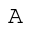
\includegraphics[width=0.2\textwidth]{train_set00}}
    \fbox{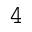
\includegraphics[width=0.2\textwidth]{train_set01}}
    \fbox{
\includegraphics[width=0.2\textwidth]{train_set02}}
    \caption{Extrait du jeu d'images initial}
\end{figure}

Cependant, ce type d'apprentissage induit un certain biais sur les valeurs
puisque ce n'est pas notre OCR qui a traité les caractères, il n'y a donc pas
toute la partie pré-traitement et découpage qui va modifier grandement le
résultat des images.

Nous avons donc rapidement changé d'approche en générant à la place des PDF de
plusieurs dizaines de pages remplies de caractères, dans plusieurs polices
d'écriture. Chaque page du PDF est ensuite convertie en image PNG, et donnée en
entrée à notre logiciel d'OCR pour passer sur les multiples phases
(pré-traitement puis segmentation) avant d'arriver au réseau.

\begin{figure}[H]
    \centering
    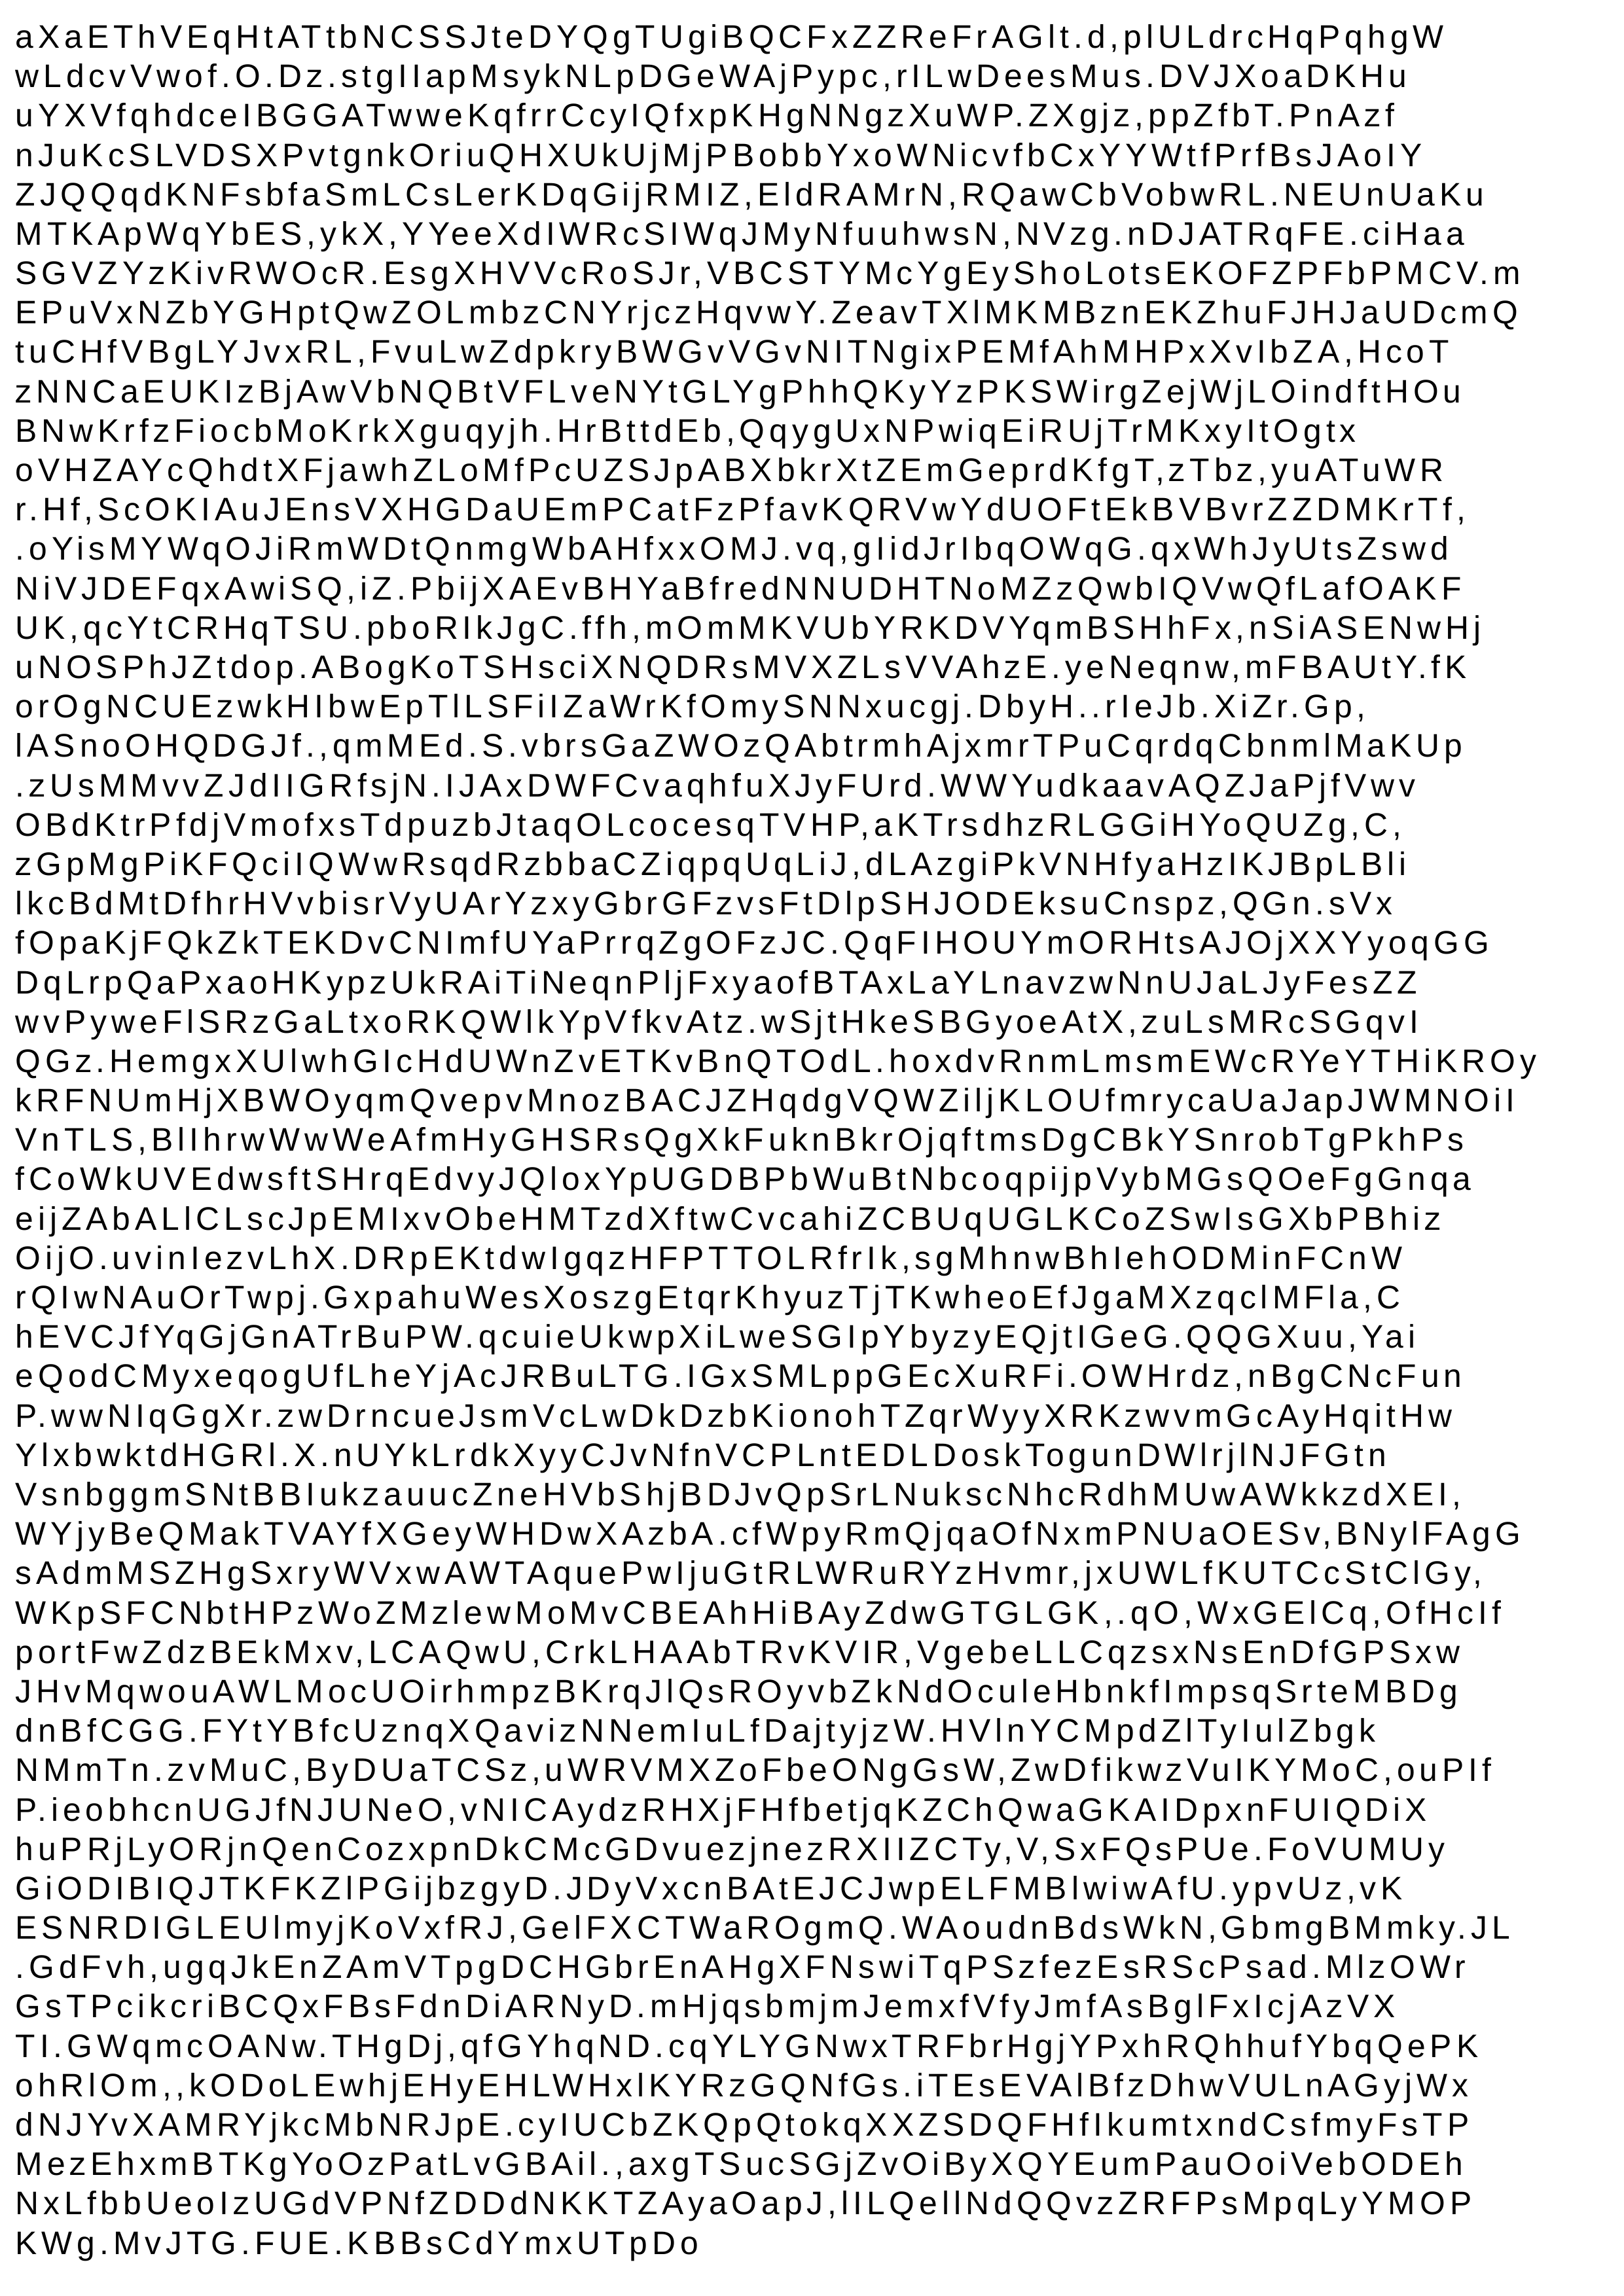
\includegraphics[width=0.5\textwidth]{new_dataset}
    \caption{Extrait du jeu d'images final}
\end{figure}

Nous avons décidé d'utiliser trois polices d'écriture différentes lors de
l'apprentissage : Liberation Sans, Liberation Serif, et Liberation Mono. Ces
dernières sont les équivalents libres des trois polices les plus utilisées des
systèmes Microsoft à savoir : Arial, Times New Roman, et Courier New. Au total
ce sont presque 100000 caractères dans chaque police d'écriture qui sont
générés, et constituent le jeu de données final. Le jeu d'entraînement comprend
60\% des données, celui de validation 20\% et celui de test 20\%.

Ajouter davantage de police aurait permis à notre réseau de mieux généraliser
les différentes écritures, mais cela représente surtout un apprentissage bien
plus long et difficile à ajuster.

\section{Sauvegarde et chargement}

Il est possible de sauvegarder et charger les poids et biais de chaque couche
d'un réseau depuis un fichier. Ceci permet d'éviter de devoir entraîner le
réseau à nouveau, et facilite grandement les tests lors de l'apprentissage. De
même, cette fonctionnalité de sauvegarde et chargement a été implémentée pour
les jeux de données ce qui a permis un gain de temps énorme pendant la phase
d'expérimentation de l'apprentissage.

Le format pour stocker ces informations est sous forme binaire pour compresser la
taille du fichier résultant.

Pour le réseau de neurones :

\begin{minted}{text}
    nb_couches
    taille_couche1 taille_couche2 ...
    matrice_poids_couche1
    matrice_biais_couche1
    ...
\end{minted}

Pour un jeu de données :

\begin{minted}{text}
    nb_exemples
    matrice_entree_ex1
    matrice_sortie_ex1
    ...
\end{minted}

\section{Évaluation}

Pour contrôler le réseau lors de son apprentissage, nous avons mis en place
diverses fonctions de monitoring pour calculer à chaque époque de l'algorithme
du gradient la précision du réseau et le coût sur les jeux de données
d'entraînement et de validation.

\begin{minted}[fontsize=\footnotesize]{text}
    datasets sizes:
    full_set: 283500
    train_set: 170100
    validation_set: 56700
    test_set: 56700

    training network with parameters:
    layers size: [1024, 30, 54]
    nb_examples: 170100
    nb_epochs: 10
    mini_batch_size: 10
    learn_rate: 0.001000
    regularization_rate: 5.000000

    done epoch 1
    train_set results:
    accuracy: 42.00%
    cost: 4.55
    validation_set results:
    accuracy: 42.00%
    cost: 4.56

    done epoch 2
    train_set results:
    accuracy: 72.00%
    cost: 3.99
    validation_set results:
    accuracy: 72.00%
    cost: 3.99

    done epoch 3
    train_set results:
    accuracy: 85.00%
    cost: 3.40
    validation_set results:
    accuracy: 85.00%
    cost: 3.41
\end{minted}

\newpage

\begin{figure}[H]
    \centering
    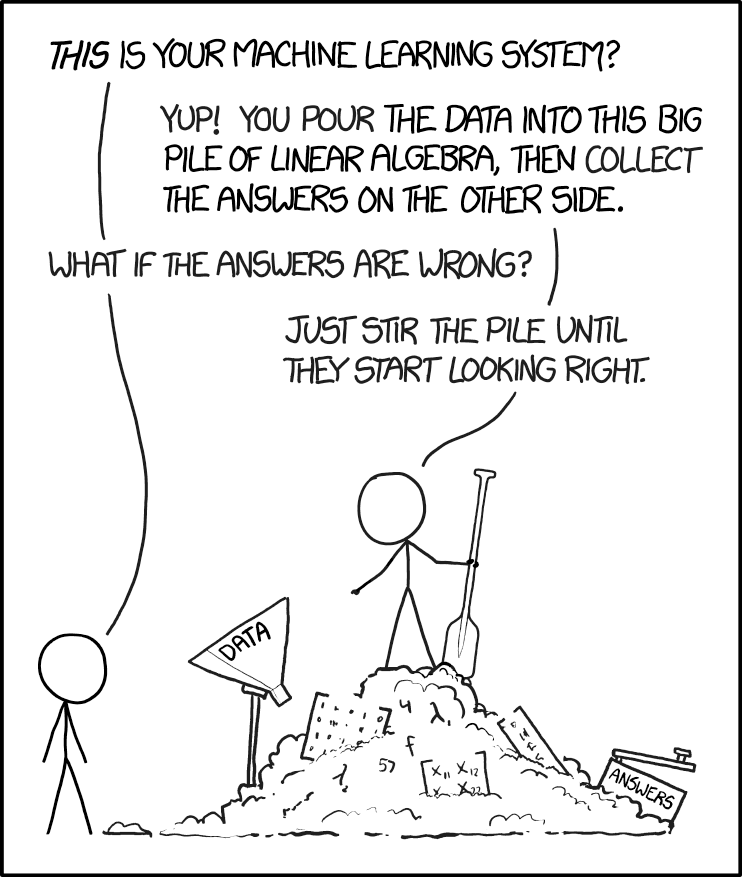
\includegraphics[width=0.8\textwidth]{xkcd_machine_learning}
    \caption*{\textit{xkcd}, Randall Munroe}
\end{figure}
